The main idea of this chapter is to introduce the different stages during the implementation. Here I will introduce the different problems and the solutions I have chosen to overcome those problems.

\todo{Introduce different sections}

%%%%%%%%%%%%%%%% 2PC POKER IMPLEMENTATION %%%%%%%%%%%%%%%%%%
%%%%%%%%%%%%%%%%%%%%%%%%%%%%%%%%%%%%%%%%%%%%%%%%%%%%%%%%%%%%
\section{The Poker Game}
This is the overall structure of every implemetation that wants to use the $Duplo$ protocol. In the next part I will introduce how this was used to implement the poker game in this project.

\bigskip

\todo{The pokser setting}
\begin{figure}
\label{poker_setting}
\centering
\begin{figure}
\label{con_swap_fig}
\centering
\begin{figure}
\label{con_swap_fig}
\centering
\begin{figure}
\label{con_swap_fig}
\centering
\input{figurs/poker_setting}
\caption{The two different settings discussed to implement. The one on the left where the $Constructor$ and the $Evaluator$ also are the players and the one on the right wher they act as servers where players connect and then localy construct output based on output from the servers.}
\end{figure}

\caption{The two different settings discussed to implement. The one on the left where the $Constructor$ and the $Evaluator$ also are the players and the one on the right wher they act as servers where players connect and then localy construct output based on output from the servers.}
\end{figure}

\caption{The two different settings discussed to implement. The one on the left where the $Constructor$ and the $Evaluator$ also are the players and the one on the right wher they act as servers where players connect and then localy construct output based on output from the servers.}
\end{figure}

\caption{The two different settings discussed to implement. The one on the left where the $Constructor$ and the $Evaluator$ also are the players and the one on the right wher they act as servers where players connect and then localy construct output based on output from the servers.}
\end{figure}


Before starting on the implemetation it was inportant to figure out which setting to study. Different settings was proposed before a choise was made. Mainly two settings were discussed. One where the $Constructor$ and $Evaluatr$ acteded as players of the poker game themselves or a setting where they acted as servers where the players connected to. The first one was the one chosen mainly because of the simplicity of doing it and timelimmet in the project. But the other setting has some nice features which I will note here. That setting resembles more what is done in online poker to day. Where a client connects to a game provider which deals the cards. Then instead of connecting to one party which is not completly trusted the player connects to two servers which runs a secret share of the protocol together. Such that th eplayer recieves a share from each party. One of these serves could be a Stat authorized server in which the palyer would put its trust. This would bring down the main part of the latency from the setting implemented in this study. Which will be discussed later. This could be done as the preprocessing of the circuit could be done on forehand and in times with low load. But this implemetation adds a complexity in the implemetation phase where message authentication codes are needed to ensure that non of the two servers changed the output. This second setting also allow for more the two player to participate in the game.

\bigskip



\todo{Describe the roles of the two parties}

\todo{why can only one hand be played at a time, broken bristol compiler ehn frigate v2 was fixed}

\todo{Describe the more interresting setting, why is it interresting and why is it not implemented}

\todo{Discuss latensy in different framework calls}

\begin{figure}
    \label{fig:mesurement_ms}
    \centering

    \begin{subfigure}{\textwidth}
        \label{fig:const_ms_plot}
        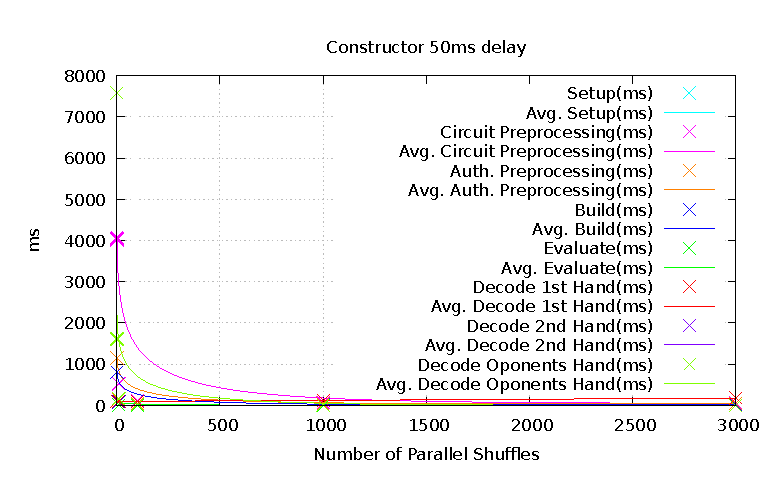
\includegraphics[width=\textwidth]{figurs/const_ms_plot.eps}
        \caption{Constructor: 50ms simulated network latency. Showing the time used in different phases per deck shuffled.}
    \end{subfigure}

    \vspace*{1cm}

    \begin{subfigure}{\textwidth}
        \label{fig:eval_ms_plot}
        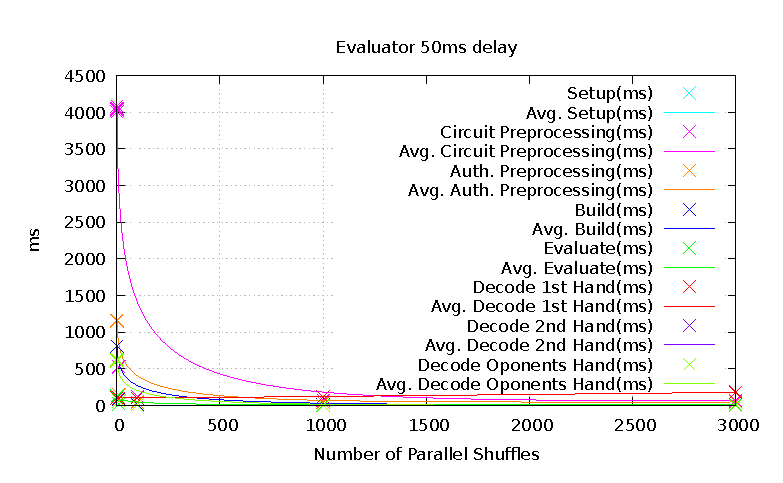
\includegraphics[width=\textwidth]{figurs/eval_ms_plot.eps}
        \caption{Evaluator: 50ms simulated network latency. Showing the time used in different phases per deck shuffled.}
    \end{subfigure}

\caption{Comparison of the Constructor and Evaluator on which phases requires the most time.}
\end{figure}

\begin{figure}
    \label{fig:mesurement_kb}
    \centering

    \begin{subfigure}{\textwidth}
        \label{fig:const_kb_plot}
        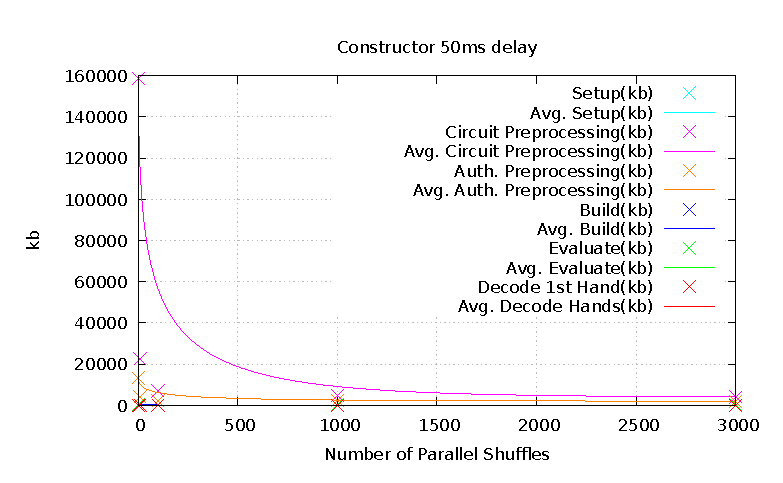
\includegraphics[width=\textwidth]{figurs/const_kb_plot.eps}
        \caption{Constructor: $kb$ sent in different phases.}
    \end{subfigure}

    \vspace*{1cm}

    \begin{subfigure}{\textwidth}
        \label{fig:eval_kb_plot}
        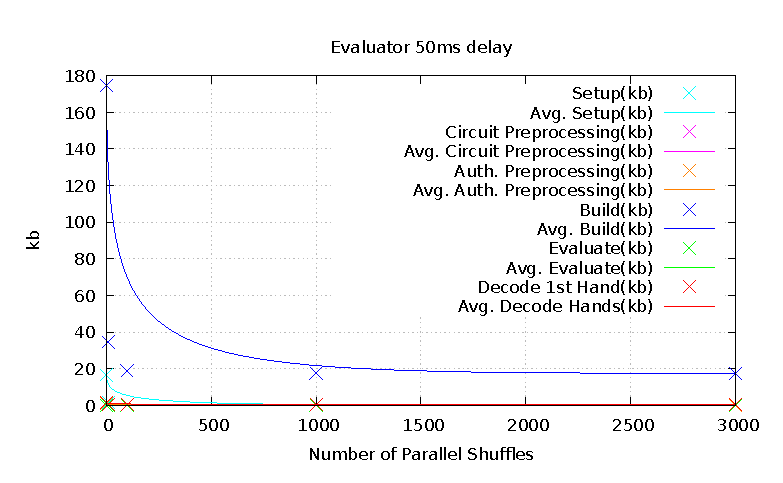
\includegraphics[width=\textwidth]{figurs/eval_kb_plot.eps}
        \caption{Evaluator: $kb$ sendt in different phases.}
    \end{subfigure}

\caption{Comparison of Constructor and Evaluator on which phases most $kb$ are sent to the other party.}
\end{figure}


\begin{table}[!htb]
\label{table:mesurement_ms}
\centering

    \begin{subtable}{\textwidth}
    \label{table:const_ms}
    \centering
    \scalebox{.7}{
    \begin{tabular}{l || c |r r r r r}
          &           & \multicolumn{5}{c}{Number of Parallel Shuffles} \\
    Phase & Delay(ms) & 1 & 10 & 100 & 1000 & 3000    \\
    \hline
    \multirow{3}{*}{Setup} & 50 & 2210.37 & 162.11 & 17.63 & 2.86 & 2.17   \\
                           &  0 & 1431.11 & 114.23 & 12.66 & 2.36 & 2.00   \\
                           \cline{2-7}
                           &  - &  779.29 &  47.88 &  4.97 & 0.50 & 0.17   \\
    \hline                       
    \multirow{3}{*}{Circuit preprocess} & 50 & 4033.93 & 527.35 & 119.99 & 67.52 & 51.36 \\
                                        &  0 & 1564.52 & 201.07 &  50.75 & 29.75 & 19.50 \\
                                        \cline{2-7}
                                        &  - & 2469.41 & 326.28 &  69.24 & 37.77 & 31.86 \\
    \hline 
    \multirow{3}{*}{Auth preprocess} & 50 & 1150.64 & 143.22 & 39.92 & 37.93 & 42.54 \\
                                     &  0 &   93.10 &  31.95 & 20.02 & 22.90 & 33.57 \\
                                     \cline{2-7}
                                     &  - & 1057.54 & 121.27 & 19.90 & 17.03 &  8.97 \\
    \hline                                 
    \multirow{3}{*}{Build} & 50 & 807.18 & 86.06 & 15.78 & 8.42 & 10.82 \\
                           &  0 &  22.84 &  6.79 &  6.27 & 6.46 &  9.02 \\
                           \cline{2-7}
                           &  - & 784.34 & 79.27 &  9.51 & 1.96 &  1.8 \\
    \hline                       
    \multirow{3}{*}{Evaluate} & 50 & 100.82 & 10.22 & 1.18 & 0.30 & 0.30 \\
                              &  0 &   0.69 &  0.24 & 0.24 & 0.23 & 0.24 \\
                              \cline{2-7}
                              &  - & 100.13 &  9.98 & 0.94 & 0.07 & 0.06 \\
    \hline
    \multirow{3}{*}{Decode keys 1st hand} & 50 & 100.37 & 100.39 & 100.91 & 115.62 & 177.92 \\
                                          &  0 &   0.20 &   0.13 &   0.37 &  10.20 &  77.15 \\
                                          \cline{2-7}
                                          &  - & 100.17 & 100.26 & 100.54 & 105.42 & 100.77 \\
    \hline
    \multirow{3}{*}{Decode keys 2nd hand} & 50 & 100.37 & 10.23 & 1.24 & 0.50 & 0.86 \\
                                          &  0 &   0.13 &  0.08 & 0.90 & 0.25 & 1.30 \\
                                          \cline{2-7}
                                          &  - & 100.24 & 10.15 & 0.34 & 0.25 & -0.44 \\
    \hline
    \multirow{3}{*}{Decode Opponents hand} & 50 & 100.35 & 10.22 & 1.23 & 0.48 & 0.57 \\
                                           &  0 &   0.11 &  0.08 & 0.09 & 0.23 & 0.91 \\
                                           \cline{2-7}
                                           &  - & 100.24 & 10.14 & 1.14 & 0.25 & -0.34
    \end{tabular}
    }
    \caption{Constructor: comparison of the different phases and concurrent shuffles with and with out delay.}
    \end{subtable}%

    \vspace*{1cm}

    \begin{subtable}{\textwidth}
    \label{table:eval_ms}
    \centering
    \scalebox{.7}{
    \begin{tabular}{l || c |r r r r r}
          &           & \multicolumn{5}{c}{Number of Parallel Shuffles} \\
    Phase & Delay(ms) & 1 & 10 & 100 & 1000 & 3000    \\
    \hline
    \multirow{3}{*}{Setup} & 50 & 620.25 & 61.89 & 6.15 & 0.62 & 0.21 \\
                           &  0 & 117.58 & 11.36 & 1.05 & 0.09 & 0.03 \\
                           \cline{2-7}
                           &  - & 502.67 & 50.53 & 5.01 & 0.53 & 0.18 \\
    \hline                       
    \multirow{3}{*}{Circuit preprocess} & 50 & 4037.57 & 528.96 & 120.39 & 68.30 & 60.86 \\
                                        &  0 & 1574.70 & 202.97 &  51.89 & 30.79 & 29.63 \\
                                        \cline{2-7}
                                        &  - & 2462.87 & 325.99 &  68.50 & 37.51 & 31.23 \\
    \hline 
    \multirow{3}{*}{Auth preprocess} & 50 & 1154.60 & 146.40 & 44.90 & 42.32 & 46.33 \\
                                     &  0 &   94.98 &  34.70 & 24.73 & 27.37 & 37.65 \\
                                     \cline{2-7}
                                     &  - & 1059.62 & 111.70 & 20.17 & 14.95 &  8.68 \\ 
    \hline                                 
    \multirow{3}{*}{Build} & 50 & 807.23 & 86.12 & 15.83 & 8.50 & 10.88 \\
                           &  0 &  22.88 &  6.82 &  6.33 & 6.59 &  9.14 \\
                           \cline{2-7}
                           &  - & 784.35 & 79.30 &  9.50 & 1.91 &  1.74 \\
    \hline                       
    \multirow{3}{*}{Evaluate} & 50 & 129.49 & 17.91 & 5.43 & 5.44 & 9.58 \\
                              &  0 &  15.71 &  5.13 & 2.92 & 2.29 & 7.96 \\
                              \cline{2-7}
                              &  - & 113.78 & 12.78 & 2.51 & 3.15 & 1.62 \\
    \hline
    \multirow{3}{*}{Decode keys 1st hand} & 50 & 100.60 & 100.63 & 101.17 & 115.91 & 179.12 \\
                                          &  0 &   0.29 &   0.19 &   0.43 &  15.01 & 125.68 \\
                                          \cline{2-7}
                                          &  - & 100.31 & 100.44 & 100.26 & 100.90 &  53.44 \\
    \hline
    \multirow{3}{*}{Decode keys 2nd hand} & 50 & 100.59 & 10.23 & 1.47 & 22.08 & 128.10 \\
                                          &  0 &   0.18 &  0.08 & 0.22 & 14.31 & 124.84 \\ 
                                          \cline{2-7}
                                          &  - & 100.41 & 10.15 & 1.25 &  7.77 &   3.26 \\
    \hline
    \multirow{3}{*}{Decode Opponents hand} & 50 & 100.57 & 10.23 & 12.70 & 21.81 & 122.89 \\
                                           &  0 &   0.17 &  0.07 &  0.22 & 14.16 & 123.14 \\
                                           \cline{2-7}
                                           &  - & 100.40 & 10.16 & 12.48 &  7.65 & -0.25
    \end{tabular}
    }
    \caption{Evaluator: comparison of the different phases and number of concurrent shuffles with and without delay.}
    \end{subtable}%

\caption{Comparison of the time consumption of the Constructor and Evaluator.}
\end{table}


\begin{table}[!htb]
\label{table:mesurmet_kb}
\centering

    \begin{subtable}{\textwidth}
    \label{table:const_kb}
    \centering
    \scalebox{1}{
    \begin{tabular}{l || r r r r r}
                                & \multicolumn{5}{c}{Number of Parallel Shuffles} \\
    Phase                       &         1 &       10 &     100 &    1000 & 3000 \\
    \hline
    Setup                       &     12.70 &     1.27 &    0.12 &    0.01 &    0.00 \\
    Circuit Preprocess          & 158470.00 & 22518.10 & 7023.94 & 4837.94 & 4127.91 \\
    Auth. Preprocess            &  13329.90 &  4170.08 & 2249.69 & 2437.49 & 1986.51 \\
    Build                       &    327.71 &   128.49 &  107.24 &  105.12 &  104.96 \\
    Evaluate                    &    122.84 &   122.84 &  122.84 &  122.48 &  122.84 \\
    Decode keys                 &      5.94 &     2.38 &    2.02 &    1.99 &    1.99\\
    \end{tabular}
    }
    \caption{Constructor: $kb$ sent per shuffled deck in different phases.}
    \end{subtable} 
    
    \vspace*{1cm}
    
    \begin{subtable}{\textwidth}
    \label{table:eval_kb}
    \centering
    \scalebox{1}{
    \begin{tabular}{l || r r r r r}
                                & \multicolumn{5}{c}{Number of Parallel Shuffles} \\
    Phase                       &         1 &       10 &     100 &    1000 & 3000 \\
    \hline
    Setup                       &  16.55 &  1.65 &  0.17 &  0.02 &  0.01 \\
    Circuit Preprocess          &   1.59 &  0.16 &  0.02 &  0.00 &  0.00 \\
    Auth. Preprocess            &   1.06 &  0.11 &  0.01 &  0.00 &  0.00 \\
    Build                       & 174.55 & 34.67 & 18.95 & 17.55 & 17.49 \\
    Evaluate                    &   0.11 &  0.10 &  0.10 &  0.10 &  0.10 \\
    Decode keys                 &   1.44 &  0.58 &  0.49 &  0.48 &  0.48 
    \end{tabular}
    }
    \caption{Evaluator: $kb$ sent per shuffled deck in different phases.}
    \end{subtable}%

\caption{Comparison of the Constructor and Evaluator on the amount of data sent in the different phases.}
\end{table}